The finite element approach presented in this research can be extended to analyse the compression of surfaces in AFM imaging. Spherical and periodic structures provide the simplest structures to consider. These structures were modelled as three-dimensional, homogeneous elastic parts with elastic modulus and Poisson ratio comparable to biomolecules. The simulations focused on the compression produced when scanning along the centre axis of the structures, generating 2D force and indentation data over the restricted central axis. Subsequently, the radial compression of spherical samples and distortion in periodic structures are analysed as a function of the indentation force. This elucidates the responses and characteristics produced in the surfaces under AFM imaging and the apparent appearance of the structure.   

\subsubsection{Analysis of Hemisphere Structure}

As presented in Figure \ref{fig: Hemisphere Compression Plot}, the hemisphere simulations provided 2D heat maps of the indention force across a surface cross-section. This displays the force experienced at each depth along the scan line. The raw data from the simulation, shown in \ref{fig: Hemisphere-ContourPlotNI-1}, produces a course-grained distribution of indentation force over the scan. Using interpolation methods detailed in Section \ref{Chapter 2: Quantitative Analysis of Surface Compression}, the data can be smoothed to produce a continuous distribution shown in Figure \ref{fig: Hemisphere-ContourPlotI-1}. From the raw data, contours of constant force can be extracted to analyse the perceived shape at varying forces as presented in Figure \ref{fig: Hemisphere-LineContour-1}.

\begin{figure}[H]
\centering
        
    \begin{subfigure}[t]{0.325\textwidth}
        \centering
        \caption{\label{fig: Hemisphere-ContourPlotNI-1} }
        \vspace{-0.1in}
             \begin{tikzpicture}
                \node (img1) {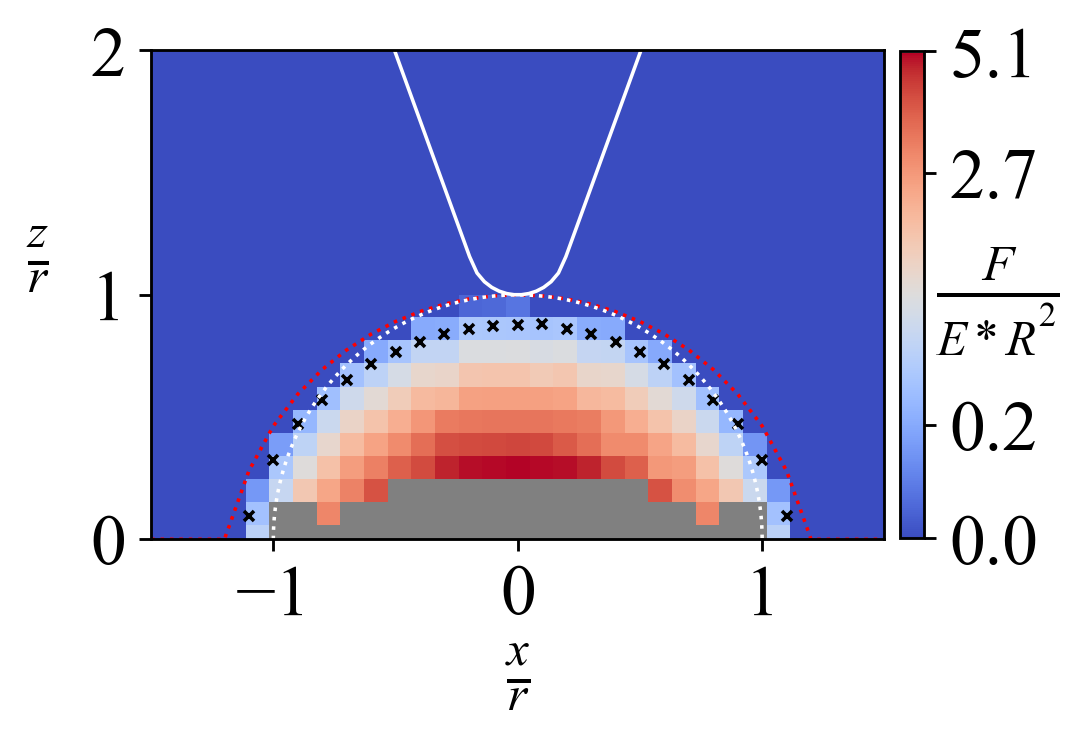
\includegraphics[trim = 41.5 55.5 55 10, clip, width=0.95\linewidth]{Figures/Hemisphere-ContourPlotNI-1.png}};
                \node (img2) at ([xshift=1cm,yshift=-1cm]img1.north west) [scale=0.25] {\includegraphics[width=1\linewidth]{Figures/Axis.png}};
              \end{tikzpicture}
    \end{subfigure}
    \hfill
    \begin{subfigure}[t]{0.325\textwidth}
        \centering
        \caption{\label{fig: Hemisphere-ContourPlotI-1} }
        \vspace{-0.1in}
             \begin{tikzpicture}
                \node (img1) {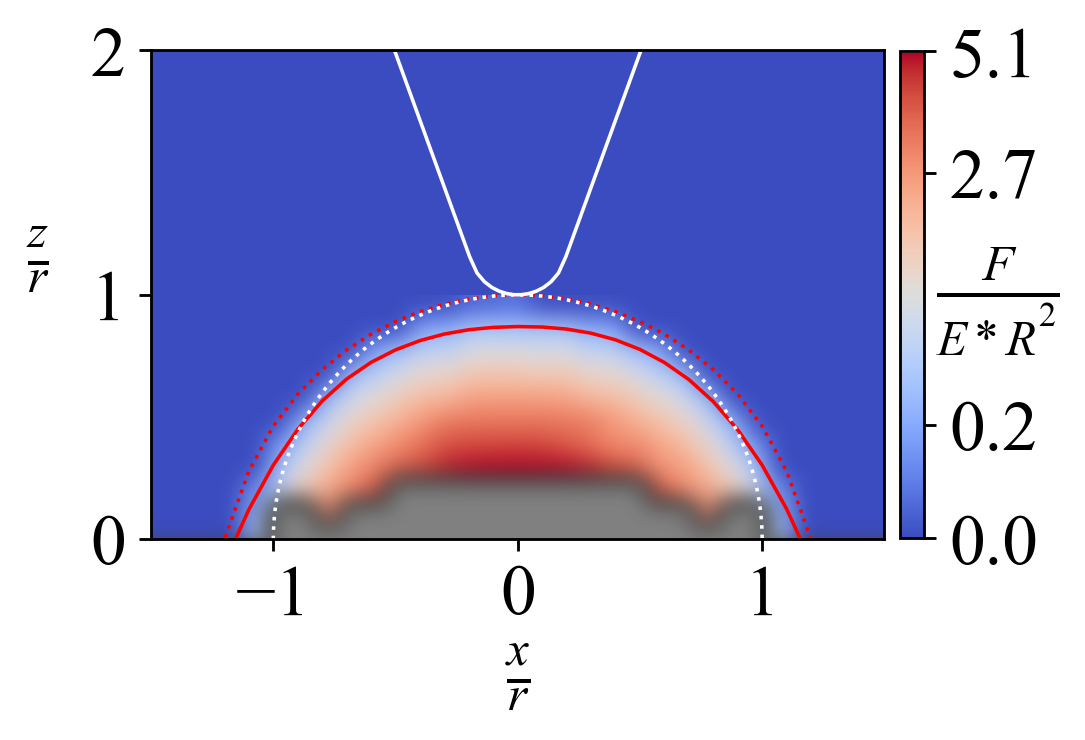
\includegraphics[trim = 41.5 55.5 55 10, clip, width=0.95\linewidth]{Figures/Hemisphere-ContourPlot-1.png}};
                \node (img2) at ([xshift=1cm,yshift=-1cm]img1.north west) [scale=0.25] {\includegraphics[width=1\linewidth]{Figures/Axis.png}};
              \end{tikzpicture}
    \end{subfigure}
    \hfill
    \begin{subfigure}[t]{0.325\textwidth}
        \centering
        \caption{\label{fig: Hemisphere-LineContour-1} }
        \vspace{-0.1in}
             \begin{tikzpicture}
                \node (img1) {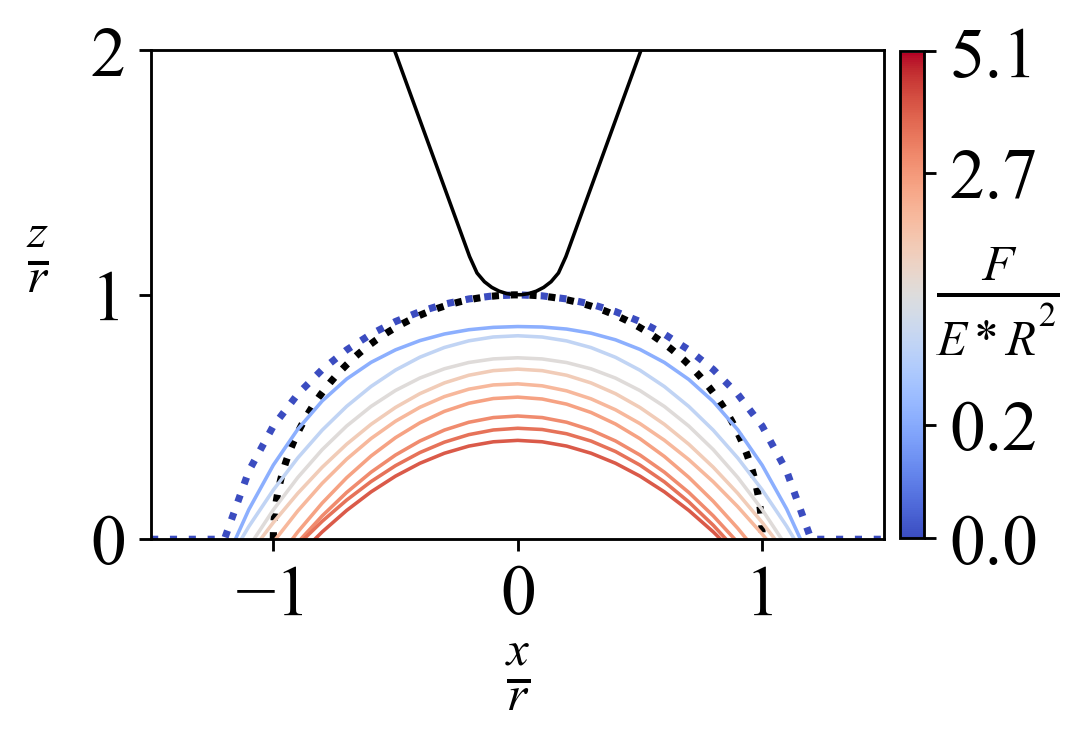
\includegraphics[trim = 41.5 55.5 55 10, clip, width=0.95\linewidth]{Figures/Hemisphere-LineContour-1.png}};
                \node (img2) at ([xshift=1cm,yshift=-1cm]img1.north west) [scale=0.25] {\includegraphics[width=1\linewidth]{Figures/Axis.png}};
              \end{tikzpicture}
    \end{subfigure} 
    \caption{\label{fig: Hemisphere-ContourPlot}Illustrations of data produced from compression simulations for indenter $R/r=0.2$. (A) Raw two-dimensional heat map of indentation force over the scanning axis for the hemisphere structure. Including the points of constant force, $\frac{F}{E^*R^2} = 0.227 $, shown as black crosses. These are points used to produce the force contours. The indenter is solid white, and the surface is dotted white. Points of zero force/ hard sphere contact is shown in dotted red. (B) Interpolated two-dimensional heat map of indentation force over the scanning axis for the hemisphere structure. Including overlayed contour of constant force, $\frac{F}{E^*R^2} = 0.227 $, shown in solid red. The indenter is solid white, and the surface is dotted white. Points of zero force/ hard sphere contact is shown in dotted red. (C) Two-dimensional plot of force contours for varying indentation/ reference forces over the scanning axis of the hemisphere structure. Force shown varies within the limit of $ 0.227 < \frac{F}{E^*R^2} < 3.867 $. The indenter and surface are black, with the initial zero force/ hard sphere boundary in dashed blue.}
    
\end{figure}

Analysis of the compression, shown in Figure \ref{fig: Hemisphere-ContourPlot-1} and \ref{fig: Hemisphere-ContourPlot-7}, revealed that increasing the indenter-to-surface ratio results in lower indentation forces. As the surface-indenter ratio/contact radius increases, the forces are spread over a larger area, resulting in less deformation for the same force. Combined with greater tip convolution, this increases the broadening of the surface's appearance. This is reflected in fitted Young's modulus as shown in Figure \ref{fig: Hemisphere-Youngs}. As indentation force, and therefore fitted Young's modulus, varies as a function of the contact radius, the variation in Young's modulus over the scan position emulates the scan geometry. Therefore, larger indenters produce a flatter fitted Young's modulus. This highlights that increasing the indenter-surface ratio is analogous to scanning a surface with greater Young's modulus. Physically, this corresponds to greater effective stiffness experienced at larger indenter-surface ratios, as forces are distributed over a larger surface area and larger forces are required for equivalent compression. Interestingly, due to the flattening produced, larger indenter-surface ratios provide a greater estimation of the true Young's modulus over the scan positions.

\begin{figure}[ht]
\centering

    \begin{subfigure}[t]{0.295\textwidth}
        \centering
        \caption{\label{fig: Hemisphere-Setup} }
        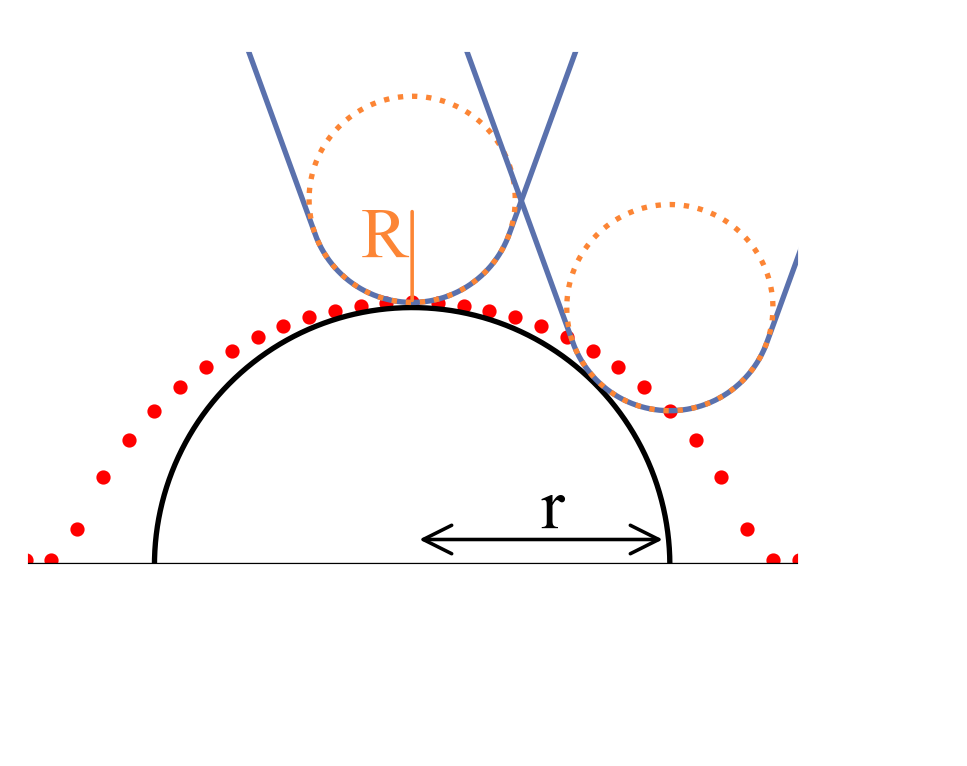
\includegraphics[width=1\linewidth]{Figures/Hemisphere-SetUp.png}
    \end{subfigure}
    \hfill
    \begin{subfigure}[t]{0.345\textwidth}
        \centering
        \caption{\label{fig: Hemisphere-ContourPlot-1} }
        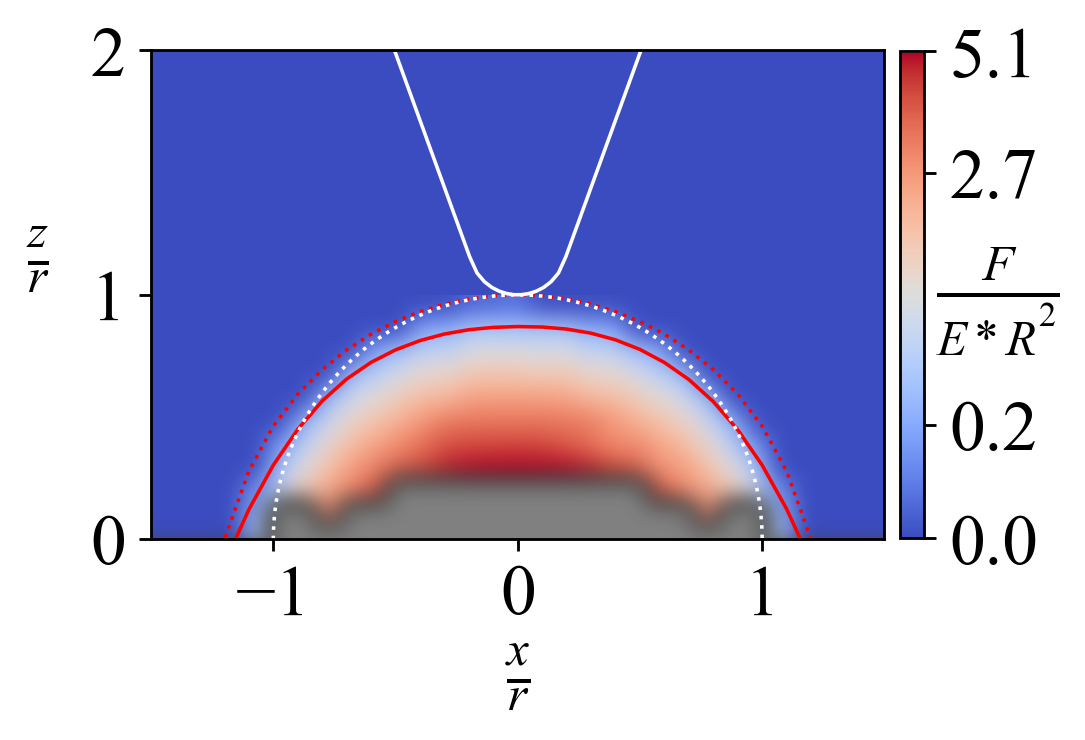
\includegraphics[width=1\linewidth]{Figures/Hemisphere-ContourPlot-1.png}
    \end{subfigure}
    \hfill
    \begin{subfigure}[t]{0.345\textwidth}
        \centering
        \caption{\label{fig: Hemisphere-ContourPlot-7} }
        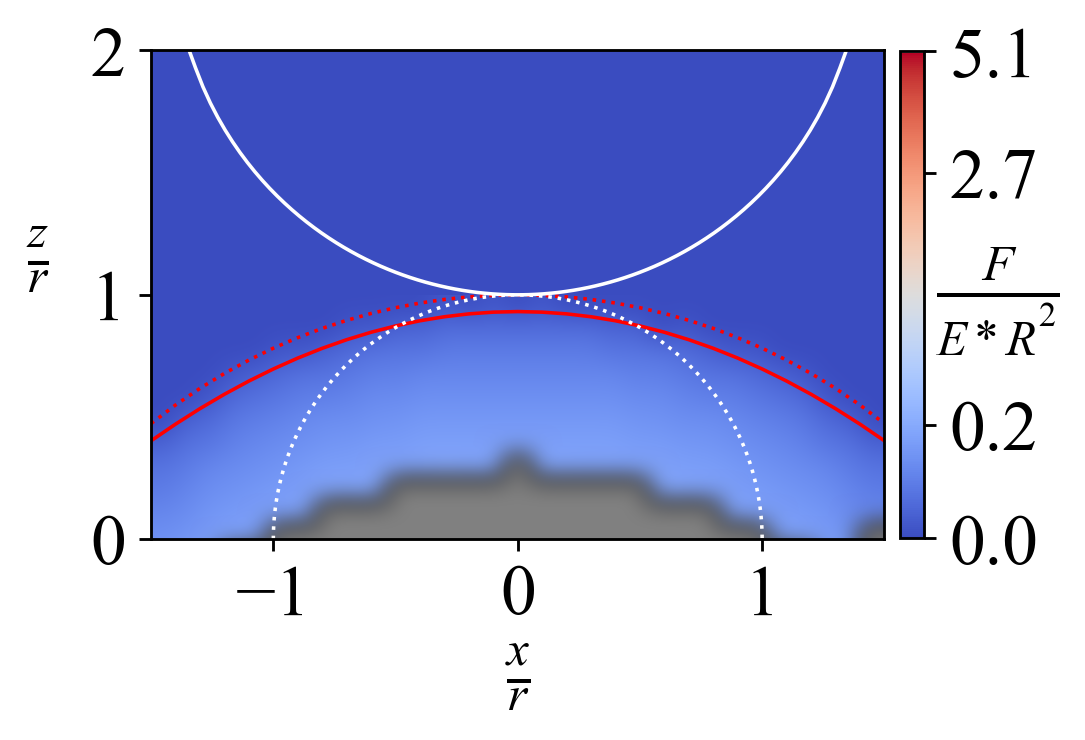
\includegraphics[width=1\linewidth]{Figures/Hemisphere-ContourPlot-7.png}
    \end{subfigure}


    \hfill
    \vspace{-0.3in}
     
    
    \begin{subfigure}[t]{0.325\textwidth}
        \centering
        \caption{\label{fig: Hemisphere-Youngs} }
        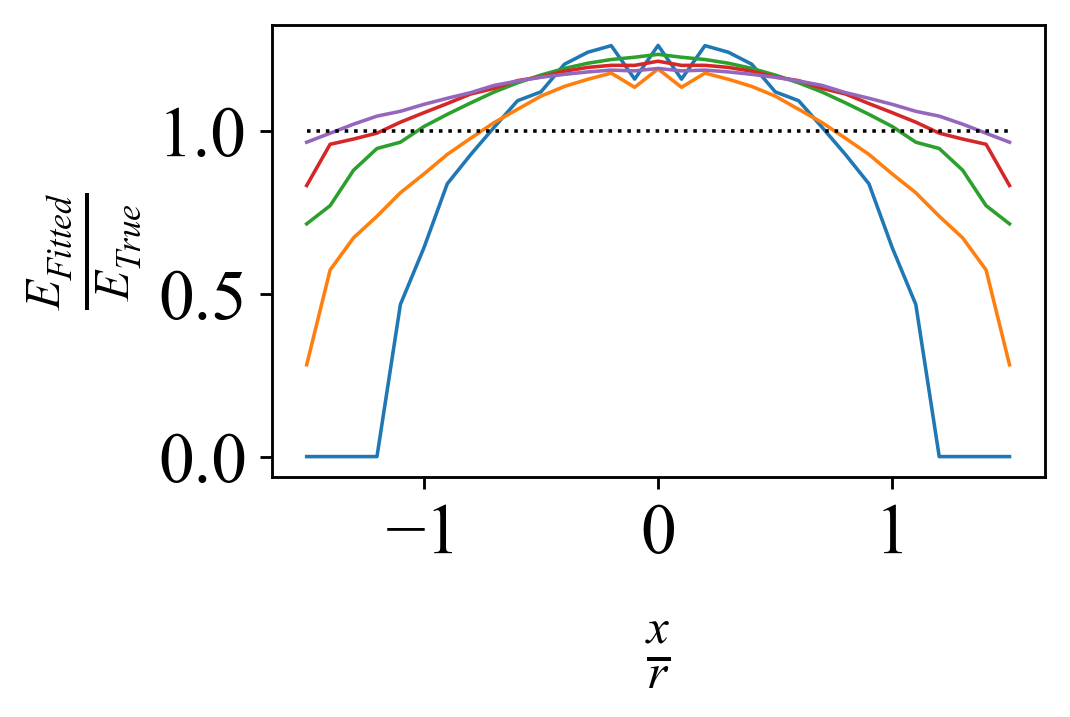
\includegraphics[width=1\linewidth]{Figures/Hemisphere-Youngs.png} 
    \end{subfigure}
     \hfill
    \begin{subfigure}[t]{0.325\textwidth}
        \centering
        \caption{\label{fig: Hemisphere FWHM} }
        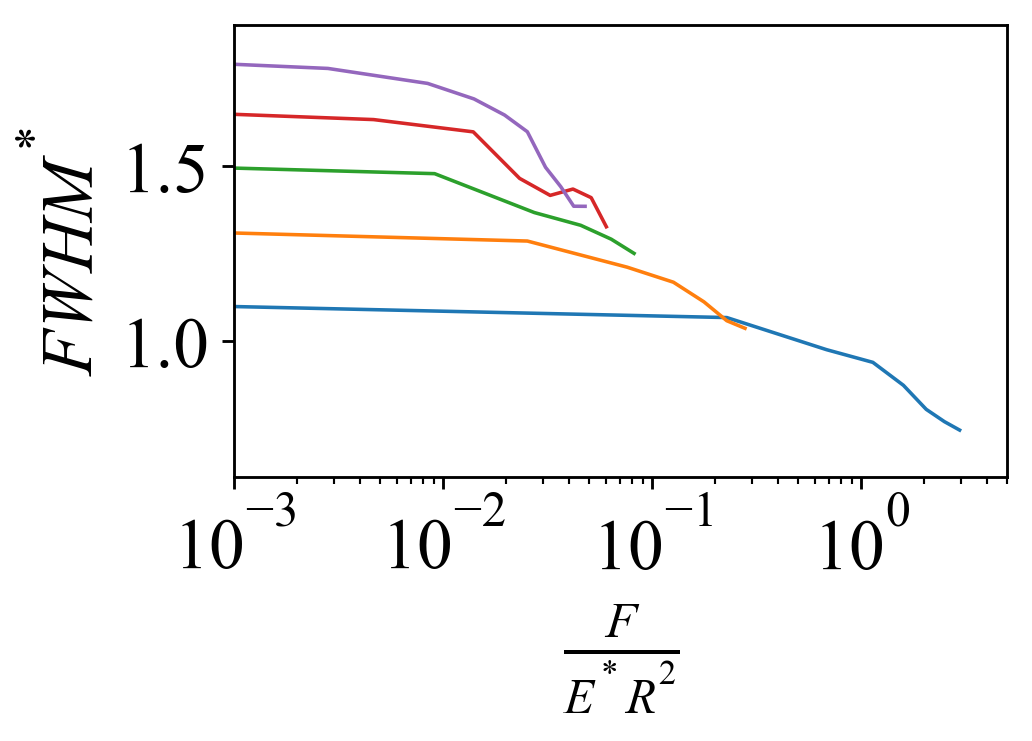
\includegraphics[width=1\linewidth]{Figures/Hemisphere-FWHM.png}
    \end{subfigure}
     \hfill
    \begin{subfigure}[t]{0.325\textwidth}
        \centering
        \caption{\label{fig: Hemisphere-Volume} }
        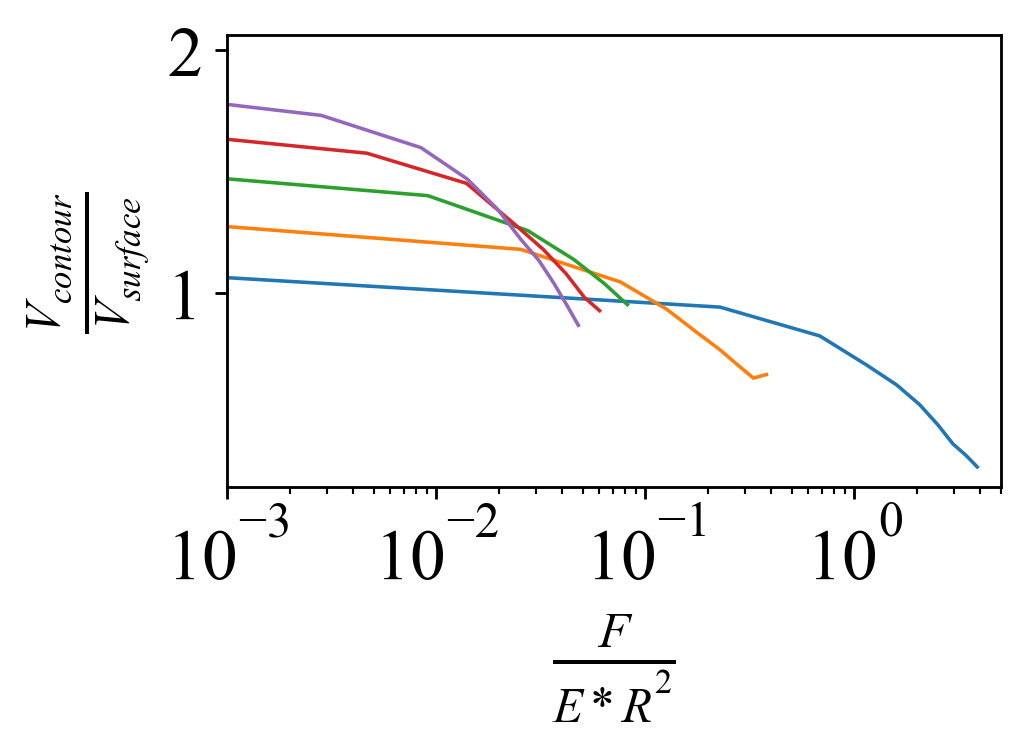
\includegraphics[width=1\linewidth]{Figures/Hemisphere-Volume.png}
    \end{subfigure}

     \hfill
     
    \begin{subfigure}[t]{1\textwidth}
        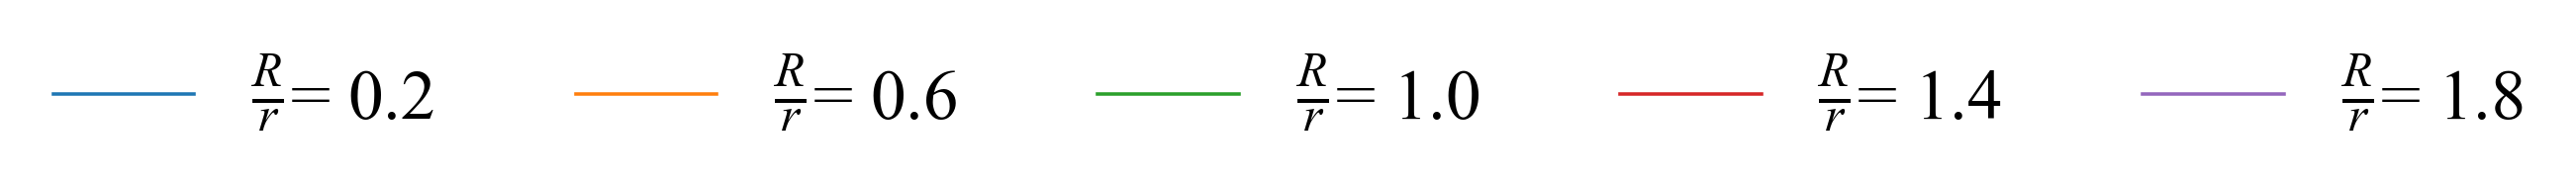
\includegraphics[width=1\linewidth]{Figures/Hemisphere-Legend.png}
    \end{subfigure}
    
    \caption{\label{fig: Hemisphere Compression Plot}(A) Geometry of scan along the central axis of a hemisphere. Three-dimensional geometry is produced by rotating the indenter and semi-circle around the central z-axis. The hemisphere is shown in black with a radius $r$. Indenter geometry is shown in blue, with the circular tip of radius $R$ in orange. Red points indicate initial scan positions (Hard sphere contact points). (B) Interpolated two-dimensional heat map of indentation force over the scanning axis for hemisphere structure with indenter $R/r=0.2$. Including overlayed contour of constant force, $\frac{F}{E^*R^2} = 0.227 $, shown in solid red. The indenter is solid white, and the surface is dotted white. Points of zero force/ hard sphere contact is shown in dotted red. (C) Interpolated two-dimensional heat map of indentation force over the scanning axis for hemisphere structure with indenter $R/r=1.4$. Including overlayed contour of constant force, $\frac{F}{E^*R^2} = 0.227 $, shown in solid red. The indenter is solid white, and the surface is dotted white. Points of zero force/ hard sphere contact is shown in dotted red. (D) Fitted Young's modulus over scan positions for each indenter radius ($R/r$). (E) Relative FWHM of the contour divided by FWHM of true geometry ($FWHM^*=\frac{FWHM}{FWHM_{True}}$) variation over contour force for each indenter radius($R/r$). (F)  Volume variation over contour force in spherical structures for each indenter radius($R/r$).}
    
\end{figure}

The Full Width Half Maxima (FWHM) provides information about the spread of the contour. The FWHM value reflects the surface's compression and is used as an indicator flattening of the contour. As shown in Figure \ref{fig: Hemisphere FWHM}, FWHM decreases asymptotically as the indentation force decreases. As the force decreases to zero, each indenter converges on the corresponding FWHM of the hard sphere boundary. Conversely, as the force increases, the sample is indented to greater depth producing tighter, compressed force contours and narrowing the surface's appearance. For larger indenters, this produces force contours with FWHM closer to the true FWHM. However, this does not directly show that the higher force provides a more accurate recreation of the sample surface. The compression of the sample can produce elliptical contours that do not represent the hemisphere yet share the same FWHM. For a smaller indenter, which approximates the surface geometry more closely at low force, the increased compression at higher forces produces an FWHM that diverges from the true surface FWHM. Furthermore, the nonlinear behaviour of the FWHM highlights that the compression producing the force contours is not a simple linear relationship. 

Furthermore, the apparent volume can quantify compression over various contour forces. As shown in Figure \ref{fig: Hemisphere-Volume}, the volume decreases exponentially as the indentation force increases. This further validates the behaviour shown by the FWHM. As the indentation force increases, greater compression is produced, reducing the apparent appearance. In addition, as indenter size decreases, larger forces are required to achieve the same relative decrease in volume. This is expected as smaller indenters have smaller contact areas; therefore, larger forces are required to compress the sample to the same extent.

Overall, this analysis highlights three main characteristics of the hemisphere under compression. First, the Youngs modulus shows the dependence of elastic response/behaviour on the contact radius and tip convolution. The FWHM is an important analysis to demonstrate the nonlinear compression and widening of the perceived surface. Finally, the volume highlights that the larger indenters/contact areas require larger forces to compress the sample to the same extent as smaller indenters.